\documentclass[conference]{IEEEtran}
\IEEEoverridecommandlockouts
\usepackage{cite}
\usepackage{amsmath,amssymb,amsfonts}
\usepackage{graphicx}
\usepackage{textcomp}
\usepackage{xcolor}
\usepackage{booktabs}
\usepackage{multirow}
\usepackage{tikz}
\usetikzlibrary{arrows.meta,positioning,fit,calc}
\usepackage[hidelinks]{hyperref}

\definecolor{colCo}{HTML}{DCE8F5}
\definecolor{colBG}{HTML}{F6C89F}
\definecolor{colBa}{HTML}{BFE3C8}
\definecolor{colRo}{HTML}{E2D5EE}

\graphicspath{{../figures/}{figures/}}
\makeatletter
\def\input@path{{../tables/}{tables/}{../figures/}{figures/}}
\makeatother

\begin{document}

\title{Dual-View Address Mapping for NPU--PIM Memory on Ramulator~2.0}

\author{\IEEEauthorblockN{Yash Gupta}
\IEEEauthorblockA{Roll No. 264101064\\
Dept. of Computer Science and Engineering\\
IIT Guwahati\\
\texttt{yash.g@iitg.ac.in}}
\and
\IEEEauthorblockN{Nikunj Ladumor}
\IEEEauthorblockA{Roll No. 264101032\\
Dept. of Computer Science and Engineering\\
IIT Guwahati\\
\texttt{nikunj.ladumor@iitg.ac.in}}
\and
\IEEEauthorblockN{Vamshi Kumar Kanduri}
\IEEEauthorblockA{Roll No. 264101061\\
Dept. of Computer Science and Engineering\\
IIT Guwahati\\
\texttt{vamshi.kanduri@iitg.ac.in}}
\and
\IEEEauthorblockN{Priyanshu Ganjeer}
\IEEEauthorblockA{Roll No. 264101035\\
Dept. of Computer Science and Engineering\\
IIT Guwahati\\
\texttt{priyanshu.ganje@iitg.ac.in}}}

\maketitle

\begin{abstract}
An NPU and a processing-in-memory (PIM) unit that share one DRAM want different physical layouts of the same weight matrix: the NPU streams the matrix and needs consecutive accesses spread over independent DRAM resources, while all-bank PIM needs the parallel PIM units to sit in different banks over the same input range. PFM~\cite{zhao2026pfm} chooses one jointly optimized layout per 2\,MB page with a mixed-integer linear program (MILP). We reproduce this optimizer for the weight shapes of LLaMA3-8B. A PuLP/CBC MILP assigns the 15 line-index bits of a 2\,MB page to column, bank-group, bank and row bits of a DDR4 device under capacity and structural constraints, maximizing $\mathrm{NPU}(f)+\alpha\,\mathrm{PIM}(f)$. We add a region-aware address mapper to Ramulator~2.0 that gives every 2\,MB region its own layout. We compare NPU-friendly, PIM-friendly and jointly optimized layouts: NPU sequential-read utilization is simulated in Ramulator, and PIM matrix-vector (GEMV) utilization is computed with an analytical all-bank model driven by Ramulator's DDR4-2400 timings. Over all seven weight matrices of a decoder layer, the optimized layout with $\alpha{=}0.25$ keeps 93.8\% NPU utilization (NPU-friendly: 95.2\%) while raising PIM utilization from 18.6\% to 48.1\%; with $\alpha{=}2$ it reaches 96.1\% PIM utilization (PIM-friendly: 71.3\%). For \texttt{down\_proj}, both fixed layouts (designed for $d_{\mathrm{in}}{=}4096$) give 4\% PIM utilization and the optimizer recovers 48--96\%. We also show that on single-channel DDR4 no layout can be best for both devices at once, and explain why.
\end{abstract}

\begin{IEEEkeywords}
processing-in-memory, NPU, DRAM address mapping, LLM inference, integer linear programming, Ramulator
\end{IEEEkeywords}

\section{Introduction}
LLM inference mixes compute-bound phases (prefill, batched GEMM) with memory-bound phases (decode-time GEMV). Recent systems pair an NPU for the former with near-bank PIM for the latter~\cite{heo2024neupims,seo2024ianus,park2024attacc}. When both share one memory, the weight matrices exist only once, so they have one physical layout. The two devices want different layouts~\cite{zhao2026pfm,seo2025facil}:
\begin{itemize}
\item The \textbf{NPU} reads a matrix as one sequential stream. It is fast when consecutive bursts go to independent resources (channels, or bank groups in DDR4) so that the data bus never waits.
\item \textbf{All-bank PIM}~\cite{lee2021hbmpim,he2020newton} sends one command to all banks; each bank's PIM unit processes a different output column over the same input slice. This needs the units' columns in \emph{different banks} and each column's data in as few rows as possible.
\end{itemize}
PFM~\cite{zhao2026pfm} solves this with a \emph{dual-view} memory: one physical layout per 2\,MB page, chosen by a MILP that scores how well a layout serves each device.

\textbf{Task.} We implement the PFM address-mapping optimizer for one tensor shape in Python with PuLP~\cite{mitchell2011pulp}, add a mapping choice per memory region to Ramulator~2.0~\cite{luo2024ramulator2}, and compare three layouts for the LLaMA3-8B~\cite{llama3} weight matrices: NPU-friendly, PIM-friendly and jointly optimized. We report bandwidth utilization for sequential NPU reads and for PIM GEMV. GPU kernels, hardware synthesis and larger models are out of scope.

\textbf{Contributions.}
(1) A verified MILP that maps 15 address bits to DDR4 levels and matches the best of 20,000--100,000 random layouts in every case.
(2) \texttt{PFMRegionMapper}, a new Ramulator~2.0 address mapper that holds a table of layouts and selects one per 2\,MB region, checked to give cycle-identical results to an independent Python bit permutation, and a utilization metric checked against Ramulator's own throughput counter.
(3) Measurements on all seven LLaMA3-8B weight matrices for DDR4 x8 and x16, an $\alpha$ sweep, and a bound that explains why one layout cannot serve both devices fully on single-channel DDR4.

\section{Background}
\subsection{DRAM organization and timing}
A DDR4 address selects a row, a column, a bank and a bank group~\cite{jedec79_4}. A read to the open row of a bank is a row hit; a read to another row needs precharge and activate ($t_{RP}+t_{RCD}=16+16$ cycles for DDR4-2400R). Two reads to the \emph{same} bank group must be $t_{CCD\_L}=6$ cycles apart; reads to \emph{different} bank groups only $t_{CCD\_S}=4$ cycles. A 64\,B burst (BL8) occupies the bus for 4 cycles, so a stream that stays in one bank group can reach at most $4/6=66.7\%$ of the bus bandwidth. On DDR4 the bank-group bits therefore play the role that channel bits play in the HBM system of the paper.

\subsection{Address mapping}
A mapping assigns each physical-address bit to one DRAM level. Inside a 2\,MB page of 64\,B lines there are $2^{21}/2^{6}=2^{15}$ lines, i.e.\ 15 free bits. For DDR4\_8Gb\_x8 (4 bank groups $\times$ 4 banks) they split into 7 column, 2 bank-group, 2 bank and 4 row bits; for x16 (2 bank groups) into 7, 1, 2 and 5.

\subsection{Weight layout and the PIM unit window}
We compute $y=xW$ with FP16 weights stored column by column, so one column of $W$ is $d_{\mathrm{in}}\cdot 2$\,B $= 2^{p_n}$ lines ($p_n{=}7$ for $d_{\mathrm{in}}{=}4096$; $p_n{=}9$ for $d_{\mathrm{in}}{=}14336$ padded to 16384). Line $\ell = c\cdot 2^{p_n} + t$ holds offset $t$ of column $c$. With $U$ PIM units (one per bank: $U{=}16$ for x8, $U{=}8$ for x16), unit $u$ processes columns $c = U g + u$. The bits that select the unit are therefore line-index bits $p_n \ldots p_n+\log_2 U - 1$, which we call the \emph{unit window}. All-bank PIM runs at full speed only if every unit-window bit is a bank-group or bank bit.

\section{Method}
\begin{figure}[t]
\centering
\resizebox{\columnwidth}{!}{%
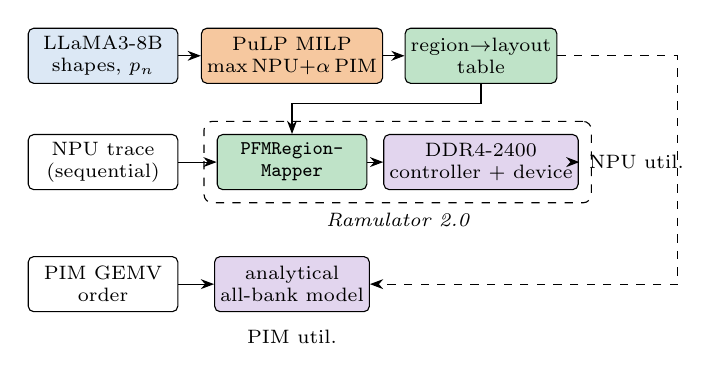
\begin{tikzpicture}[font=\scriptsize,
  box/.style={draw, rounded corners=2pt, align=center, minimum height=7mm, minimum width=19mm, inner sep=2pt, fill=#1},
  box/.default=white, >=Stealth]
\node[box=colCo] (shape) at (0,0) {LLaMA3-8B\\shapes, $p_n$};
\node[box=colBG] (milp) at (2.4,0) {PuLP MILP\\$\max \mathrm{NPU}{+}\alpha\,\mathrm{PIM}$};
\node[box=colBa] (tab) at (4.8,0) {region$\rightarrow$layout\\table};
\node[box] (npu) at (0,-1.35) {NPU trace\\(sequential)};
\node[box=colBa] (map) at (2.4,-1.35) {\texttt{PFMRegion-}\\\texttt{Mapper}};
\node[box=colRo] (ctl) at (4.8,-1.35) {DDR4-2400\\controller + device};
\node[box] (pim) at (0,-2.9) {PIM GEMV\\order};
\node[box=colRo] (model) at (2.4,-2.9) {analytical\\all-bank model};
\node[draw, dashed, rounded corners=3pt, fit=(map)(ctl), inner sep=1.6mm,
      label={[font=\scriptsize\itshape]below:Ramulator 2.0}] {};
\draw[->] (shape) -- (milp);
\draw[->] (milp) -- (tab);
\draw[->] (tab.south) -- ++(0,-0.25) -| (map.north);
\draw[->] (npu) -- (map);
\draw[->] (map) -- (ctl);
\draw[->] (pim) -- (model);
\node[anchor=west] (o1) at (6.05,-1.35) {NPU util.};
\draw[->] (ctl) -- (o1);
\draw[->, dashed] (tab.east) -- (7.3,0) |- (model.east);
\node[below=1mm of model] {PIM util.};
\end{tikzpicture}}
\caption{Flow. The MILP picks a layout per tensor class; inside Ramulator, \texttt{PFMRegionMapper} maps every 2\,MB region with its own layout. The PIM model uses the same layout table.}
\label{fig:flow}
\end{figure}

Fig.~\ref{fig:flow} shows the flow. The experiments are about 700 lines of Python; the mapper is about 150 lines of C++.

\subsection{Per-region mapping and simulator setup}
A layout is a list of (level, bit count) pairs from the least significant line-index bit upward, e.g.\ \texttt{bg1 col6 bank1 col1 bank1 bg1 row4}. It is a pure bit permutation (no XOR, no dropped bits).

\textbf{\texttt{PFMRegionMapper}.} We added a new address-mapper implementation to Ramulator~2.0 (one C++ file registered with the controller's \texttt{addr\_mapper} interface, plus one line in \texttt{CMakeLists.txt}; the Python wrapper is generated by Ramulator). Its parameters are \texttt{region\_bits} (21 for 2\,MB), a list of \texttt{layouts}, a \texttt{region\_layout} table with one layout id per region, and a \texttt{default\_layout} for regions outside the table ($-1$ = stock RoBaRaCoCh). For each request it takes the line index, splits it into a region number and 15 local bits, sends every local bit to the DRAM level and bit position given by that region's layout, and places the region number above the layout's row bits. At start-up it checks that every layout gives the column, bank-group and bank levels exactly their device bit counts. Weights of the same $d_{\mathrm{in}}$ share one layout.

\textbf{Independent check.} We also implemented the same permutation in Python: it rewrites each address so that Ramulator's stock RoBaRaCoCh mapper decodes the intended fields, and asserts that all $2^{15}$ lines map to distinct addresses. For all 20 layouts and both access patterns, the two paths give identical cycle counts (Section~\ref{sec:region}).

Ramulator~2.0 runs one DDR4-2400R channel (DDR4\_8Gb\_x8 or x16, one rank) with FR-FCFS scheduling, open-row policy and all-bank refresh. For the Python path we located the RoBaRaCoCh field positions (x8: column [12:6], bank group [14:13], bank [16:15], row [32:17]) and verified them by simulation (Fig.~\ref{fig:bg}). Every run also asserts that the trace has no duplicate addresses and that all reads reach DRAM.

\textbf{Metric.} NPU utilization $=4\,N_{\mathrm{reads}}/\mathrm{cycles}$, with cycles in DRAM clocks. On 8192 plain sequential reads this gives 65.9\%, identical to Ramulator's reported throughput divided by the 19.2\,GB/s peak (12{,}659.6\,MB/s / 19{,}200\,MB/s).

\subsection{MILP formulation}
Binary variable $x_{l,j}=1$ if line-index bit $j\in\{0..14\}$ selects level $l\in\{\mathrm{Co},\mathrm{BG},\mathrm{Ba},\mathrm{Ro}\}$. Following PFM:
\begin{align}
\textstyle\sum_{l} x_{l,j} &= 1 \quad \forall j &&\text{(structural)}\\
\textstyle\sum_{j} x_{l,j} &= B_l \quad \forall l &&\text{(capacity)}
\end{align}
\textbf{NPU score.} A bank-group bit at position 0 makes consecutive reads alternate bank groups ($t_{CCD\_S}$); a row bit below a column bit makes a sequential sweep reopen rows:
\begin{equation}
\mathrm{NPU}(f) = \tfrac{2}{3} + \tfrac{1}{3}x_{\mathrm{BG},0} - \lambda \frac{\sum_{i<j} z_{ij}}{B_{\mathrm{Ro}}B_{\mathrm{Co}}},\quad z_{ij}\ge x_{\mathrm{Ro},i}+x_{\mathrm{Co},j}-1,
\end{equation}
with $\lambda=0.25$; $2/3$ and $1$ are the bus rates under $t_{CCD\_L}$ and $t_{CCD\_S}$.

\textbf{PIM score.} Let $k$ be the number of bank-group or bank bits and $r$ the number of row bits in the unit window of width $w=\log_2 U$. With $k<w$, $2^{w-k}$ units share each bank and serialize; row bits in the window add row switches:
\begin{equation}
\mathrm{PIM}(f) = 2^{-(w-k)}\cdot 0.5^{\,r}.
\end{equation}
This term is made linear with a one-hot binary $y_{k,r}$ over all feasible $(k,r)$ pairs. The objective is $\max\ \mathrm{NPU}(f)+\alpha\,\mathrm{PIM}(f)$ plus a $10^{-4}$ tie-break that pushes row bits up.

\textbf{Verification.} For every solve we check that (a) the MILP objective equals an exact Python evaluation of the returned layout (catches linearization errors) and (b) it is at least as good as the best of 20,000 random layouts (100,000 in the first model). Both held in all cases. Re-running the solver reproduces every stored layout exactly.

\subsection{PIM GEMV model}
Stock Ramulator~2.0 has no PIM commands, so PIM utilization comes from an analytical model that uses Ramulator's DDR4-2400R values. Each step issues one all-bank column command: units $u=0..U{-}1$ read offset $t$ of their current column. A unit costs $t_{CCD\_L}=6$ cycles, plus $t_{RCD}=16$ if its bank has no open row or $t_{RP}+t_{RCD}=32$ if the row changes. Units in the same bank add up, and the step lasts as long as the slowest bank. Utilization is the ideal time ($6$ cycles per step) over the modeled time. As a cross-check, we also replay the same access order as ordinary reads through Ramulator (the ``read-stream proxy'').

\subsection{Layouts compared}
\textbf{NPU-friendly}: BG lowest, then Co, Ba, Ro. \textbf{PIM-friendly}: Co lowest, then BG, Ba, Ro. \textbf{PFM}: the MILP solution for $\alpha\in\{0.25,1,2\}$ and each $p_n$. Table~\ref{tab:layouts} and Fig.~\ref{fig:layouts} list them.

\input{layouts_table.tex}

\begin{figure}[t]
\centering
\resizebox{\columnwidth}{!}{\input{layouts_tikz.tex}}
\caption{Bit layouts on DDR4 x8 (bit 14 left). The red box marks the PIM unit window. The PFM layouts keep a bank-group bit at bit 0 for the NPU ($\alpha{=}0.25$) or fill the window with bank-level bits ($\alpha{=}1$); for $d_{\mathrm{in}}{=}14336$ they move row bits out of the window.}
\label{fig:layouts}
\end{figure}

\section{Results}
\subsection{Bank-group interleaving decides NPU bandwidth}
\begin{figure}[t]
\centering
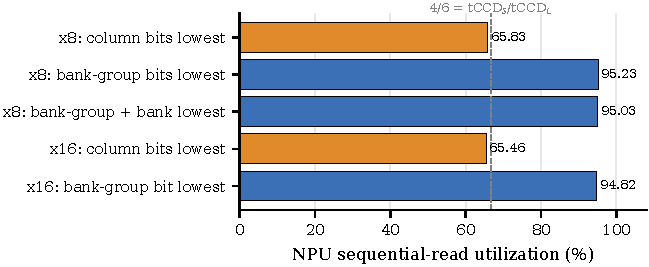
\includegraphics[width=\columnwidth]{bg_effect.pdf}
\caption{NPU sequential-read utilization in Ramulator for simple layouts. With column bits lowest every read stays in one bank group and pays $t_{CCD\_L}$; one bank-group bit at the bottom is enough to reach 95\%.}
\label{fig:bg}
\end{figure}
Fig.~\ref{fig:bg} shows the basic effect. With column bits lowest, utilization is 65.8\% (x8) and 65.5\% (x16), just under the $4/6$ bound; with a bank-group bit lowest it is 95.2\% and 94.8\%. Row hits stay above 99\% in both cases, so the loss comes from $t_{CCD\_L}$, not from row misses. Adding bank bits below the bank-group bits gives nothing (95.0\%) and three times more row conflicts. One bank-group bit is enough because two alternating groups already space same-group reads by 8 cycles $>t_{CCD\_L}$.

\subsection{Baselines}
\begin{figure*}[t]
\centering
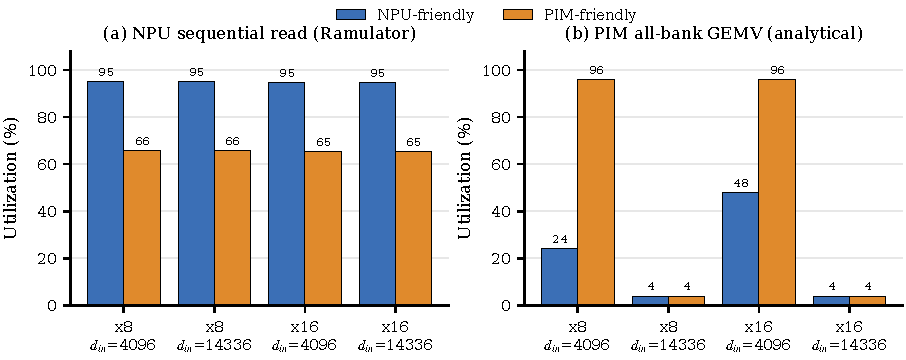
\includegraphics[width=\textwidth]{baseline.pdf}
\caption{Baselines. (a) NPU sequential read in Ramulator; (b) PIM GEMV, analytical model. Each fixed layout serves one device only, and for $d_{\mathrm{in}}{=}14336$ neither serves PIM.}
\label{fig:baseline}
\end{figure*}
Fig.~\ref{fig:baseline} shows the two fixed layouts. NPU-friendly reaches 95\% NPU utilization but only 24\% PIM utilization on x8 with $d_{\mathrm{in}}{=}4096$: two of its four unit-window bits are column bits, so four units share each bank. PIM-friendly reaches 96\% PIM but only 66\% NPU. For $d_{\mathrm{in}}{=}14336$ ($p_n{=}9$) the unit window moves up to bits 9--12, which in both fixed layouts contain two row bits. Four units then share a bank \emph{and} use different rows, so every access is a row switch and PIM utilization falls to 3.95\%. Note that both fixed layouts are designed for $d_{\mathrm{in}}{=}4096$; a PIM-friendly layout designed by hand for $d_{\mathrm{in}}{=}14336$ would move the row bits out of bits 9--12, which is what the optimizer does for $\alpha\ge1$.

\subsection{Jointly optimized layouts}
\begin{figure*}[t]
\centering
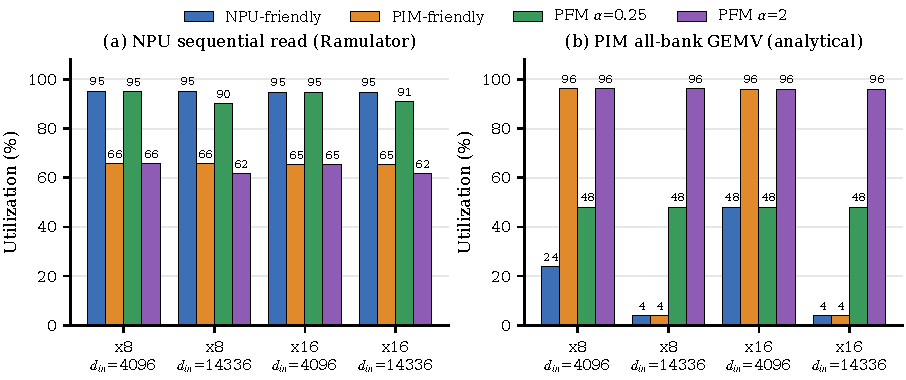
\includegraphics[width=\textwidth]{contribution.pdf}
\caption{All layouts. PFM with $\alpha{=}0.25$ keeps NPU utilization near the NPU-friendly layout and doubles (x8, $d_{\mathrm{in}}{=}4096$) or multiplies by 12 ($d_{\mathrm{in}}{=}14336$) the PIM utilization; $\alpha{=}2$ gives the best PIM utilization in every case.}
\label{fig:contribution}
\end{figure*}
\input{results_table.tex}

Fig.~\ref{fig:contribution} and Table~\ref{tab:results} add the MILP layouts.
\begin{itemize}
\item \textbf{$d_{\mathrm{in}}{=}4096$ (six matrices).} PFM $\alpha{=}0.25$ keeps the bank-group bit at position 0 and puts the other three bank-level bits in the unit window: 95.2\% NPU (same as NPU-friendly) with 48.1\% PIM instead of 24.0\%. For $\alpha\ge1$ the solver picks a layout equivalent to PIM-friendly (only the order of bank-level bits inside the window differs), with the same utilization.
\item \textbf{$d_{\mathrm{in}}{=}14336$ (\texttt{down\_proj}).} PFM moves two row bits to positions 7--8 (the top of the within-column offset) and fills the window with bank-level bits. With $\alpha{=}0.25$ it gets 90.2\% NPU and 48.1\% PIM; with $\alpha\ge1$ 96.1\% PIM at 61.7\% NPU. Both fixed layouts give 3.95\% PIM. The read-stream proxy agrees in direction (51.7\% $\rightarrow$ 94.9\%). Much of this gain comes from adapting the layout to the column length, which a hand-tuned PIM layout for this shape could also do; the optimizer's added value here is that it finds the shape-specific layout automatically and, for $\alpha{=}0.25$, one that also keeps 90\% NPU utilization.
\item \textbf{x16} shows the same pattern (Table~\ref{tab:results}).
\end{itemize}

\begin{figure}[t]
\centering
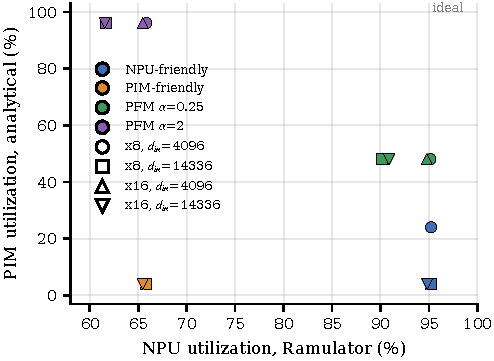
\includegraphics[width=\columnwidth]{tradeoff.pdf}
\caption{NPU vs.\ PIM utilization for all layouts. PFM layouts match or improve on the fixed layouts of the same case, but none reaches the top-right corner on single-channel DDR4.}
\label{fig:tradeoff}
\end{figure}

\subsection{Whole decoder layer}
\begin{figure*}[t]
\centering
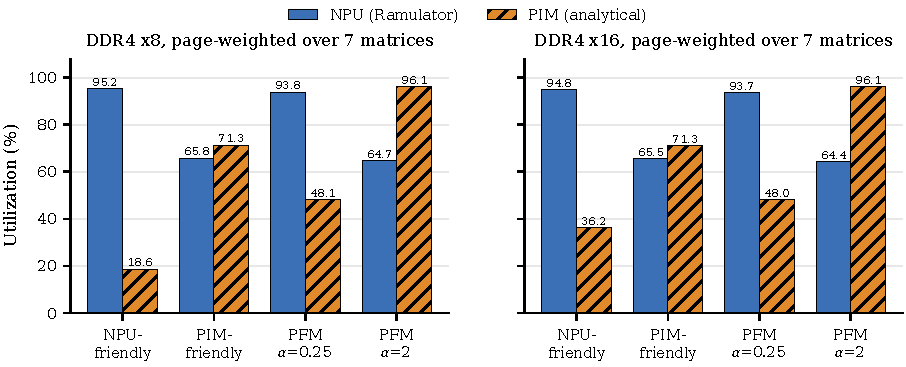
\includegraphics[width=\textwidth]{llama_weighted.pdf}
\caption{Utilization over all seven LLaMA3-8B weight matrices of one decoder layer, weighted by their 2\,MB pages.}
\label{fig:weighted}
\end{figure*}
\input{weighted_table.tex}
\input{shapes_table.tex}

Weighting each matrix by its pages (Tables~\ref{tab:weighted} and~\ref{tab:shapes}, Fig.~\ref{fig:weighted}): on x8, PFM $\alpha{=}0.25$ gives up 1.4 NPU points against NPU-friendly (93.8\% vs.\ 95.2\%) and gains 29.4 PIM points (48.1\% vs.\ 18.6\%). PFM $\alpha{=}2$ gains 24.8 PIM points over PIM-friendly (96.1\% vs.\ 71.3\%) for 1.1 NPU points.

\subsection{Effect of $\alpha$ and the single-layout bound}
For $d_{\mathrm{in}}{=}4096$ the solver switches from the NPU-oriented to the PIM-oriented layout between $\alpha{=}0.25$ and $\alpha{=}1$. In the model the switch is at $\alpha=2/3$, where $1+0.5\alpha = 2/3+\alpha$. A low $\alpha$ suits prefill-heavy serving, a high $\alpha$ decode-heavy serving.

No layout reaches high utilization on both devices on DDR4 x8, and this follows from the bit budget. The NPU needs one bank-group bit at position 0. The unit window needs all four bank-level bits ($w{=}4$), but x8 has only four, so with one at position 0 at most three can lie in the window ($k{\le}3$), which caps PIM at $2^{-1}=50\%$ of peak. The paper's HBM2e target~\cite{zhao2026pfm} has separate channel and pseudo-channel bits for NPU interleaving, so it does not face this conflict; this is why PFM reports high utilization on both devices and our DDR4 study shows a trade-off instead.

\subsection{Per-region mapping inside Ramulator}
\label{sec:region}
\input{region_numbers.tex}
\input{region_table.tex}
For \eqok\ of \eqall\ layouts (both DRAM parts, both $d_{\mathrm{in}}$ classes), replaying the plain NPU and PIM traces through \texttt{PFMRegionMapper} gives exactly the same cycle count as the Python permutation with RoBaRaCoCh, and the same utilization as Table~\ref{tab:results}. Table~\ref{tab:region} then uses several regions in one simulation: a single NPU stream reads eight 2\,MB regions, six holding $d_{\mathrm{in}}{=}4096$ weights and two holding \texttt{down\_proj}. With the PFM layouts the region table selects layout 0 for the first six regions and layout 1 for the last two. The $\alpha{=}0.25$ plan reaches 93.7\% NPU utilization, close to the page-weighted value of the single-region runs (93.9\%), so switching layouts between regions costs almost nothing.

\subsection{Model fidelity}
\begin{figure}[t]
\centering
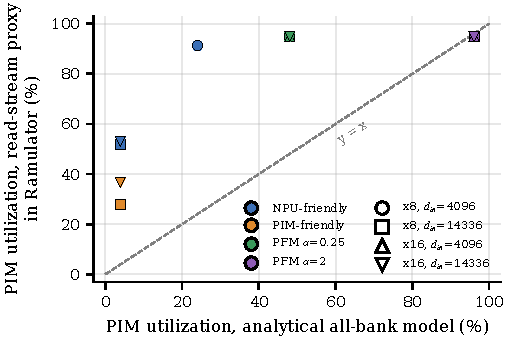
\includegraphics[width=\columnwidth]{proxy_vs_model.pdf}
\caption{Read-stream proxy in Ramulator vs.\ analytical all-bank model. FR-FCFS reorders ordinary reads and hides unit-to-bank conflicts, so the proxy is close to 95\% for most layouts.}
\label{fig:proxy}
\end{figure}
The NPU score tracks Ramulator closely: 1.00 vs.\ 95.2\%, 0.67 vs.\ 65.8\%, and 0.98 vs.\ 90.2\% (about 3 points optimistic) for the \texttt{down\_proj} layout with row bits at positions 7--8. For PIM, the read-stream proxy and the analytical model disagree (Fig.~\ref{fig:proxy}): the scheduler reorders independent reads and finds other banks, which a lock-step all-bank PIM command cannot do. We therefore report the analytical model for PIM and keep the proxy as a lower-fidelity check.

\section{Limitations}
\begin{enumerate}
\item PIM utilization is analytical, not simulated. The optimizer's PIM score and the model share the assumption that unit-window bits must be bank-level bits, so their agreement shows consistency rather than independent validation.
\item The memory is single-channel DDR4, not multi-channel HBM2e-PIM; bank-group bits stand in for channel bits, and the paper's numbers (its Table~III) are not reproduced.
\item The fixed baselines are the usual NPU-friendly and PIM-friendly orders for $d_{\mathrm{in}}{=}4096$; for \texttt{down\_proj} they are weak, so the gain there partly reflects shape adaptation rather than joint optimization.
\item Layouts are static per tensor class; there is no runtime scheduler, no address-translation hardware and no validation against real hardware.
\end{enumerate}

\section{Conclusion}
We reproduced the PFM address-mapping optimizer as a verified PuLP MILP and evaluated it on the LLaMA3-8B weight shapes with Ramulator~2.0. A new Ramulator address mapper, \texttt{PFMRegionMapper}, gives every 2\,MB region its own layout and reproduces an independent Python implementation cycle for cycle. The jointly optimized layouts improve PIM utilization at nearly the same NPU utilization (18.6\%$\rightarrow$48.1\% at 93.8\% NPU over a decoder layer), and they turn \texttt{down\_proj} from unusable for PIM (4\%) into 48--96\%. On single-channel DDR4 the bit budget forces a trade-off that $\alpha$ selects. Next steps are multiple channels and PIM commands inside Ramulator for a cycle-level PIM timing model. Source code: \url{https://github.com/groupiitg/PFM}.

\bibliographystyle{IEEEtran}
\bibliography{refs}

\end{document}
